% !TEX encoding = UTF-8 Unicode
\documentclass[a4paper, titlepage, portuguese]{article}
\usepackage[margin=2.5cm]{geometry}
%\usepackage{fontspec} % XeLaTeX
\usepackage[T1]{fontenc} % LaTeX
\usepackage[utf8]{inputenc} % LaTeX
\usepackage{newtxmath, newtxtext}
\usepackage{csquotes}
\usepackage{babel}
%\usepackage[backend=bibtex]{biblatex}
%\usepackage[backend=biber]{biblatex}
%\addbibresource{bibliography.bib}

\usepackage{indentfirst}
\usepackage{graphicx}
	\graphicspath{{images/}}
\usepackage{grffile}
\usepackage{float}
\usepackage[tableposition=top]{caption}
\usepackage{amsmath}
	%\allowdisplaybreaks
\usepackage[arrowdel]{physics}
\usepackage{esint}
\usepackage{siunitx}
	\sisetup{inter-unit-product =\ensuremath{.}, output-complex-root=\ensuremath{j},
		complex-root-position=before-number}
\usepackage{hyperref}

% Section styles
%\renewcommand{\thesection}{\Roman{section}}
%\renewcommand{\thesubsection}{\alph{subsection})}
%\renewcommand{\thesubsubsection}{\roman{subsubsection}.}
\renewcommand{\thesubsubsection}{\alph{subsubsection})}

% Useful commands
\newcommand{\eq}{\Leftrightarrow} % Equivalente
% Para numerar apenas uma equação
\newcommand\numberthis{\addtocounter{equation}{1}\tag{\theequation}}
\newcommand\e{\mathrm{e} }
\newcommand\jj{\mathrm{j} }

% Header and footer
\usepackage{fancyhdr}
\pagestyle{fancy}
\fancyhf{}
\lhead{Electrotecnia Teórica}
\rhead{4º Laboratório}
\lfoot{IST - MEEC}
\rfoot{Página \thepage}
\renewcommand{\headrulewidth}{1pt}
\renewcommand{\footrulewidth}{0.5pt}

% Document
\begin{document}
	\begin{titlepage}
		\center
		\textsc{\bfseries\LARGE Instituto Superior Técnico}\\[1cm] % Name of your university/college
		
\includegraphics[height=1.5cm]{IST_Logo.pdf}\\[2.5cm]

		\textsc{\large Engenharia Eletrotécnica e de Computadores}\\[0.5cm] % Major heading such as course name
		\textsc{\Large Eletrotecnia Teórica}\\[0.5cm] % Minor heading such as course title
		\textsc{\large 2017/2018 2º Semestre}\\[2cm]

		\rule{\textwidth}{1.6pt}\vspace*{-\baselineskip}\vspace*{2pt} % Thick horizontal line
		\rule{\textwidth}{0.4pt}\\[\baselineskip] % Thin horizontal line
			\textsc{\Huge \bfseries 4º Trabalho Laboratorial}\\[0.2cm]
			\bigskip
			\textsc{\large \bfseries Regimes Transitórios}\\[0.2cm]
		\rule{\textwidth}{0.4pt}\vspace*{-\baselineskip}\vspace{3.2pt} % Thin horizontal line
		\rule{\textwidth}{1.6pt}\\[6cm]

		\begin{minipage}{0.9\textwidth}
			\begin{flushleft} \large
				\begin{Large}\bfseries\textsc{Autores}\end{Large}\\[0.4cm]
				\begin{tabular}{l l l}
					Ricardo Simões	& 70389 & \normalsize ricardo.f.d.simoes@ist.utl.pt \\
					Rita Ramos			& 81616 & \normalsize rita.ramos@tecnico.ulisboa.pt \\
					João Pinheiro		& 84086 & \normalsize joao.castro.pinheiro@tecnico.ulisboa.pt \\
					João Sebastião	& 84087 & \normalsize joaofpsebastiao@tecnico.ulisboa.pt \\
				\end{tabular}
			\end{flushleft}
		\end{minipage}\\[0.5cm]

		\large \bfseries Laboratório segunda-feira, 09h30-11h30, Grupo D\\
		\large 14 de maio de 2018\\[1cm]
		\setcounter{page}{0}
	\end{titlepage}

	%\tableofcontents \newpage

	\section{Dimensionamento}
	% 2.1
	\subsection{}
	% a)
	\subsubsection{}
		\par
		Por aplicação da lei de indução no caminho $\vec{l}$ e desprezando efeitos resistivos fora da resistência temos
		\begin{align*}
			&\ointclockwise_{\vec{l}} \vec{E} \vdot \dd{\vec{l}} = - \dv{\psi_{\vec{l}}}{t} \\ \eq
			&0 + u_R(t) - u_g(t) = - \dv{\psi_{\vec{l}}}{t} \\ \eq
			&u_g(t) = Ri(t) + N \dv{\phi}{t}
		\end{align*}
		\par
		onde $N$ é o número de espiras da bobina e $\phi$ o fluxo que atravessa cada uma das espiras. Considerando o circuito linear temos ainda
		\begin{align*}
			&N \dv{\phi}{t} = L \dv{i(t)}{t} \\ \implies
			&u_g(t) = Ri(t) + L \dv{i(t)}{t} \numberthis \label{eq:trans_RL}
		\end{align*}
		\par
		Em $t = 0$ o gerador é ligado. Como $i(t)$ é uma variável de estado, pela continuidade da energia magnética na bobina, terá um regime transitório. A solução do regime transitório da corrente $i(t)$, dado por \eqref{eq:trans_RL}, é a soma do regime livre homogéneo (sem fontes) e do regime forçado estabelecido pelo gerador sinusoidal (quando $t \to \infty$), ou seja, $i(t) = i_l(t) + i_f(t)$.
		\par
		O regime forçado é então dado por
		\begin{align*}
			&\sqrt{2}U_{ef}\cos\left(\omega t + \alpha\right) = Ri_f(t) + L \dv{i_f(t)}{t}
		\end{align*}
		\par
		Em amplitudes complexas
		\begin{align*}
			&\bar{U}_g = R\bar{I}_f + \jj \omega L\bar{I}_f \\ \eq
			&\dfrac{\bar{U}_g}{\bar{I}_f} = \bar{Z} = R + \jj \omega L = Z\e^{\jj\varphi}
		\end{align*}
		\par
		onde
		\begin{align*}
			&Z = \sqrt{R + (\omega L)^2} \\
			&\varphi = \arctan\left(\dfrac{\omega L}{R}\right)
		\end{align*}
		\par
		O que nos permite finalmente resolver em ordem a $\bar{I}_f$ e $i_f(t)$
		\begin{align*}
			&\bar{I}_f = \dfrac{\bar{U}_g}{\bar{Z}} = \dfrac{\sqrt{2}U_{ef}}{Z} e^{\jj\left(\alpha - \varphi\right)} \\ \implies
			&i_f(t) = \Re{\bar{I}_f \e^{\jj \omega t}} = \Re{\dfrac{\sqrt{2}U_{ef}}{Z} \e^{\jj\left(\omega t + \alpha - \varphi\right)}} = \\ \eq
			&i_f(t) = \dfrac{\sqrt{2}U_{ef}}{Z} \cos\left(\omega t + \alpha - \varphi\right)
		\end{align*}
		\par
		em que $- \varphi = \SI{-1.46}{\radian} = \SI{-83.6}{\degree}$ é a desfasagem entre a tensão $u_g(t)$ e $i(t)$ em regime forçado.
		\par
		O regime livre é a solução da equação homogénea de \eqref{eq:trans_RL}
		\begin{align*}
			0 = R i(t) + L \dv{i(t)}{t} \numberthis \label{eq:trans_RL_hom}
		\end{align*}
		\par
		A equação diferencial em \eqref{eq:trans_RL_hom} ter uma solução do tipo exponencial e, portanto, fazendo $i(t) = \e^{st}$, a sua equação característica é
		\begin{align*}
			&0 = R\e^{st} + L\dv{\e^{st}}{t} \\ \eq
			&0 = R + Ls \\ \eq
			&s = - \dfrac{R}{L} = - \dfrac{1}{\tau}
		\end{align*}
		\par
		onde $\tau = \frac{L}{R} = \SI{0.286}{\milli\second}$ é a constante de tempo do circuito.
		\par
		A solução é então
		\begin{align*}
			i_l(t) = I \e^{st} = I \e^{-\frac{t}{\tau}}
		\end{align*}
		\par
		Onde a única constante de integração $I$ é determinada pela continuidade da corrente $i(t)$ na bobina
		\begin{align*}
			i(0^-) = i(0^+) = i_f(0^+) + i_l(0+)
		\end{align*}
		\par
		Dado que a corrente em $t < 0$ era nula e como $\alpha = \frac{\pi}{2}$
		\begin{align*}
			&0 =  \dfrac{\sqrt{2}U_{ef}}{Z} \cos\left(\omega 0 + \alpha - \varphi\right) + I \e^{-\frac{0}{\tau}} \\ \eq
			&I = - \dfrac{\sqrt{2}U_{ef}}{Z} \cos\left(- \frac{\pi}{2} - \varphi\right) = \SI{0.445}{\milli\ampere}
		\end{align*}
		\par
		Sendo o regime transitório finalmente dado por
		\begin{align*}
			&i(t) = i_f(t) + i_l(t) = \\ =
			&\dfrac{\sqrt{2}U_{ef}}{Z} \cos\left(\omega t + \alpha - \varphi\right) - \dfrac{\sqrt{2}U_{ef}}{Z} \cos\left(- \frac{\pi}{2} - \varphi\right) \e^{-\frac{t}{\tau}} \\ \eq
			&i(t) = \dfrac{\sqrt{2}U_{ef}}{Z} \left[ \cos\left(\omega t + \alpha - \varphi\right) - \cos\left(\alpha - \varphi\right)e^{-\frac{t}{\tau}}\right]
		\end{align*}

		\begin{figure}[H]
			\centering
			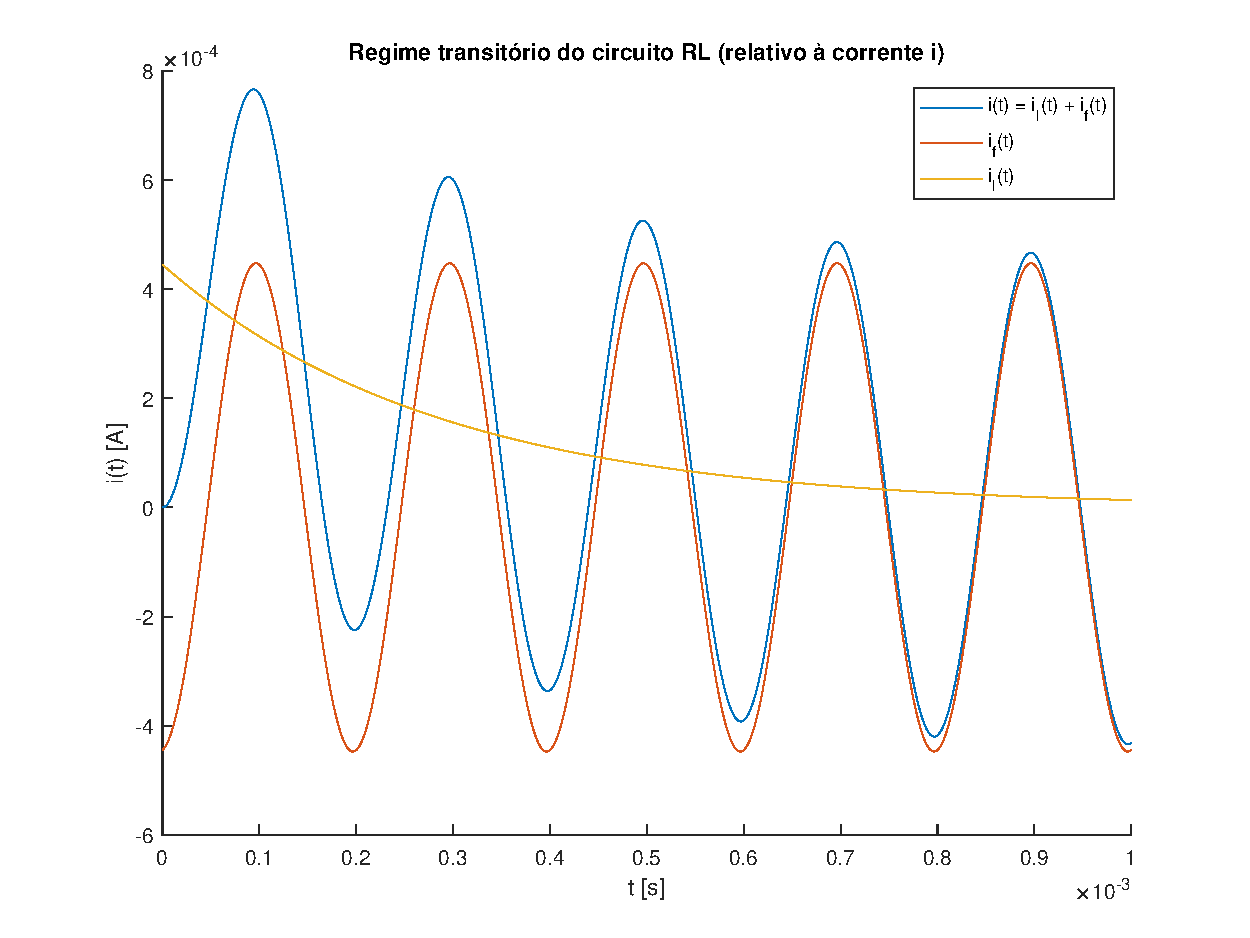
\includegraphics[width=1.0\linewidth]{rl.pdf}
			\caption{Gráfico do regime transitório da corrente $i(t)$ no circuito RL série}
			\label{fig:rl}
		\end{figure}

	% b)
	\subsubsection{}

	% c)
	\subsubsection{}
	\begin{table}[H]
		\centering
		\caption{Cinco primeiros extremos da corrente $i(t)$}
		\label{tab:extemos}
		\begin{tabular}{| r | r | S |}
			\hline
			\textbf{k} & \textbf{t} [\si{\milli\second}] & \textbf{i(t)} [\si{\milli\ampere}] \\
			\hline
			0 & 0.096 & 0.765 \\
			1 & 0.196 & -0.224 \\
			2 & 0.296 & 0.605 \\
			3 & 0.396 & -0.336 \\
			4 & 0.496 & 0.526 \\
			\hline
		\end{tabular}
	\end{table}

	% d)
	\subsubsection{}

	% e)
	\subsubsection{}

	% 2.2
	\subsection{}
	% a)
	\subsubsection{}

	%Ver \autoref{fig:figure-example}

	%\printbibliography

\end{document}
